% Setup - do not change
\documentclass[11pt]{article}
\usepackage[top=0.9in, left=0.9in, bottom=0.9in, right=0.9in]{geometry} 
\usepackage{parskip}

\usepackage[english]{babel}
\usepackage[utf8]{inputenc}
\usepackage{amsmath,amsthm,amssymb,graphicx,pdfpages,lipsum,hyperref}
\usepackage[none]{hyphenat}
\usepackage{csquotes}


% for sub figures 
\usepackage{subfigure}


\setlength\parindent{0pt}
%%%%%%%%%%%%%%%%%%%%%%%%%%%%%%%%%%%%%%%%%%%%%%%%%%%%%%%%%%%%%%%%%%%
% add other packages here if required

%% Bibliography are specified in this file. You can also choose inline bib style if you want to. But make sure your citation style is consistent (and proper)
% For more details on citation: https://library.unimelb.edu.au/recite
\usepackage[sorting = none]{biblatex}
\addbibresource{references.bib}

%%%%%%%%%%%%%%%%%%%%%%%%%%%%%%%%%%%%%%%%%%%%%%%%%%%%%%%%%%%%%%%%%%% the '%' symbol denotes comments

% Begin document creation
% DELETE THE \lipsum PLACEHOLDERS WHEN YOU BEGIN
\title{\textbf{Project 1} \\ Investigate Strategies to Improve  Yellow Taxi Driver Earnings and Company Revenue in New York City}
\author{
Jincong Chen \\
Student ID: 1264476 \\
%% Replace the link with your github repo
% 1. Remember to escape underscore (\_) in the link.
% 2. Remember to include the commit you want to submit in the link
\href{https://github.com/MAST30034-Applied-Data-Science/mast30034-project-1-jcc0026.git}{Github repo with commit}
}

\begin{document}
\maketitle

\section{Introduction}
% Link to a 30 min tutorial if you require revision: https://www.overleaf.com/learn/latex/Learn_LaTeX_in_30_minutes

As the New York City taxi industry continues to evolve in the face of changing transportation trends and market dynamics, it has become imperative for yellow taxi drivers and companies to seek innovative strategies to enhance their earnings and improve service quality. 
This report shifts its focus to New York City (NYC), aiming to explore strategies that enhance both Yellow Taxi driver earnings and company revenue. Specifically, we will concentrate on classifying pick-up hotspots, identifying high-demand periods, and investigating factors that influence driver tips. By analyzing these aspects, we seek to provide insights that simplify drivers' lives and improve their overall earnings. Additionally, our findings could offer valuable insights to taxi companies, aiding them in delivering improved services.



\section{Data}
\begin{enumerate} 
    \item The primary dataset selected for this paper originates from the \textbf{TLC Taxi Trip Record Data} \cite{TLC_taxi_data}, made publicly available by the NYC Taxi \& Limousine Commission. This dataset encompasses comprehensive trip information encompassing the entirety of completed trips within New York City's yellow taxi services.     
    For our analysis, we have decided analyse the first six month of 2018. This decision is to ensure that we capture a more complete picture of the trends and patterns in the first half year of 2018. In addition, the choice of 2018 specifically allows us to focus on a period entirely preceding the COVID-19 pandemic, eliminating the confounding effects of the pandemic-related disruptions that emerged in subsequent years. 

    In addition we will also access \textbf{taxi zone map and look up table} from the TLC Taxi Trip Record Data to supplement our geospatial analysis.

    \item A weekly gasoline fuel data from the \textbf{U.S. Energy Information Administration (EIA)} \cite{Gasoline_data} were used to supplement our analysis. The gasoline fuel dataset provides comprehensive information about weekly regular conventional retail gasoline prices in dollars per gallon across multiple states over the past decades in the US.
    

    \item Hourly weather information for New York is obtained from \textbf{Visual Crossing Weather}\cite{weather_data}. This data includes hourly measurements of temperature, wind speed, humidity, and more.

\end{enumerate}



% You can have \section{}, \subsection{}, and \subsubsection{}, \section*{}, \subsection*{}, and \subsubsection*{}
\section{Preprocessing}
\subsection{TLC taxi data}
    \subsubsection{Feature selection}
        As both ’fare\_amount’ and ’total\_amount’ are very similar and directly influence taxi driver and the company’s earning. We have decided to use ’fare amount’ as an earnings metric. This is because ’fare amount’ is solely influenced by the fare rate, trip duration, and distance, whereas 'total amount’ encompasses additional surcharges and fees which we not interest in.
        
        
        Several additional features have been ingeniously crafted to enhance the depth and scope of the analysis Such as:
        \begin{itemize}
            \item \textbf{‘Trip\_duration\_minutes’}: calculate the time difference between pickup and dropoff time in minutes. This feature can provide insights into travel patterns and time-based demand.     
            
            \item \textbf{tpep\_pickup\_datetime} into separate features
            
            \item \textbf{'pickup\_day'} to store the pickup date as date type for convenient.
            
            \item \textbf{'hour'} to store the hourly time when the trip start as integer from 0 to 23. 
            
            \item \textbf{week\_number} to store the week number of the pickup time as integer from 1 to 26 as there is maximum 27 weeks in the first 6 month of 2018.
            
            \item \textbf{'day\_of\_the\_week'} a weekday/weekend indicator attribute.
        \end{itemize}


        \subsubsection{Data cleaning/filtering}
        \begin{itemize}
            \item \textbf{Ensure records with correct time lines}. Remove any taxi record  with pickup day outside the range from 01/01/2018 to 30/06/2018.

            
            \item \textbf{Remove record with invalid 'VendorID', 'MTA\_tax', 'Extra' and 'RateCodeID'.} From the feature dictionary a valid ‘VendorID’ is value either 1 or 2, a valid ‘MTA\_tax’ is equals to \$0.50, a valid ‘Extra’ is any value in [0, 0.5, 1] and a valid ‘RateCodeID’ should be in [1,2,3,4,5,6]. 
            
            \item \textbf{Filter out invalid tip\_amount.} Remove any negative tip amount and records with positive tip amount but with payment type not credit card. 
            Assume passenger is rational that they won't give any tip amount greater than \$100. 
            
            \item \textbf{Remove invalid tolls amount.} Using the highest NYC toll of \$19 \cite{most_expensive_toll} in 2019 as a guide, and consider possible multiple toll scenarios, we have set boundary of \$38 to remove unreasonably high tolls. In addition, toll amount should be non-negative.

            \item \textbf{Remove invalid fare amount.} Using the \$3 starting charge yellow taxi in 2022\cite{start_fare} as a reference we will retain fares greater this minimum and below the 'Total\_amount' charged to passengers.
            In addition, records with fare over\$120 is very unlikely\cite{fare}, hence, will be exclude.
   

            \item \textbf{Filter invalid trip duration and trip distance.} Keep record with trip duration longer than a minute and trip distance longer than 0.2 mile. Assume passenger is rational that would not be willing to pay the initial \$3.00 fare for a ride that takes less than a minute.

            \item \textbf{Valid passenger count.} The maximum amount of passengers allowed in a yellow regular taxicab by law is 7 \cite{passenger_capacity}.

            \item \textbf{Filter Payment type.} Keep record with payment type 1 (credit card) as we will mainly be focusing the records made with card payment. 

            \item \textbf{Filter pickup location id.} As we are targeting New York's yellow taxi driver, assume drivers prefer to pickup trip within New York  hence we will ensure 'PULocationID' to be in range [1 - 263]. 

            \item  \textbf{Remove unreasonable trip duration.} Consider safe driving practices, remove trip duration longer than 2.5 hours.

            \item  \textbf{Remove any column with empty/missing value.}

        \end{itemize}
        

\subsection{Gasoline price data}
    \subsubsection{Feature selection}
        \begin{itemize}
            \item Columns that are relevant to our research are the 'date' and 'Weekly New York Regular Conventional Retail Gasoline Prices (Dollars per Gallon).
        \end{itemize}

    \subsubsection{Data cleaning/filtering}
        \begin{itemize}
            \item Remove any missing value columns
            \item By inspection of the gasoline price dataset, it is reassuring to note that all records appear to be reasonable and devoid of anomalies. Hence, no further cleaning process is necessary at this juncture.
        \end{itemize}


\subsection{Hourly Weather data}
    \subsubsection{Feature selection}
        \begin{itemize}
            \item We based on the feature dictionary, we decided to keep 'temp', 'snow', 'windspeed', 'cloudcover', 'humidity' and 'sealevelpressure, from the original data. 

            \item Similar to the taxi data, also extract new features of hour, date, and day of the week from the 'datetime' feature for analysis. 
        \end{itemize}

    \subsubsection{Data cleaning/filtering}
        \begin{itemize}
            \item Remove any missing value columns
            \item Snow depth cannot be negative 
            \item Wind speed cannot be negative 
            \item Assume temperate of a day in New York in 2018 does not exceed the maximum temperature and minimum temperature record in US
        \end{itemize}


        
\subsection{Aggregating data}
We performed various data aggregations daily, hourly, and by location (location ID), to computing average numerical values and instance counts. This approach allows us to visually explore key attributes like "trip count" and "average tip amount" across different days and locations. For instance, we aggregated weather and taxi data by pickup day and hour to analyze the relationship between weather conditions and hourly taxi demand. 

\subsection{Sampling}
Due to the large size of the yellow taxi datasets covering six months from 01/01/2018 to 30/06/2018, we have 35,960,309 records after preprocessing. Loading all this data into memory on a 16GB RAM local machine isn't feasible. Hence, we've opted to randomly sample 5\% of the data (1,798015 records) for visualization and plotting purposes.

\subsection{Transformation on categorical feature}
For categorical features like condition and day of the week, we'll use pyspark.ml's StringIndexer to map variables to label indices in an ML column.

\section{Analysis}
\subsection{Taxi data distribution}
Figure 1 displays plots of distributions of numeric features of trip duration, trip distance, tip amount and fare amount. We can see that they are all extremely right skewed. This was an indication that a transformation can be used. 

A natural logarithm transformation was used to transform these features. To avoid taking log of 0, since tip amount could potentially be zero, we will add one to all tip amount before taking the log.
% the [h] ensures your figure is inline at the location and not displayed on some other page
\begin{figure}[h]

    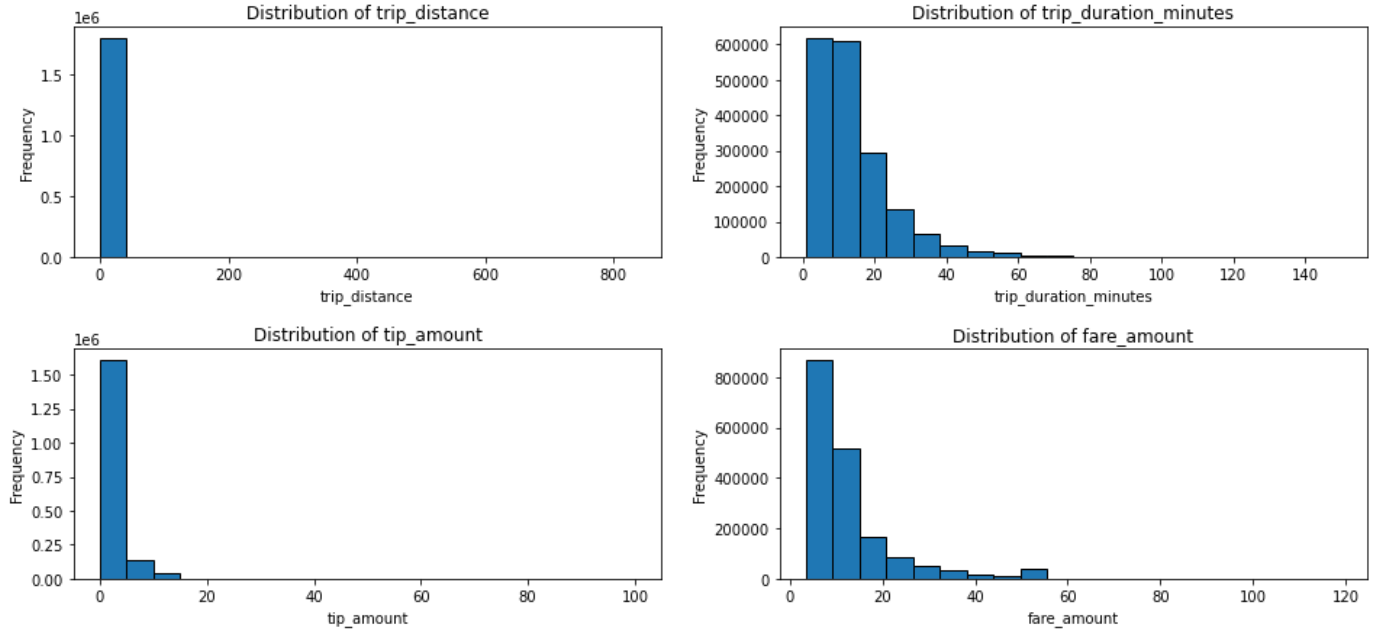
\includegraphics[width=1\textwidth]{plots/distribution.png}
    \centering
    \caption{Distribution of numeric feature in taxi data} % refer to this image as (Figure 1)
\end{figure}
\begin{figure}[h]

    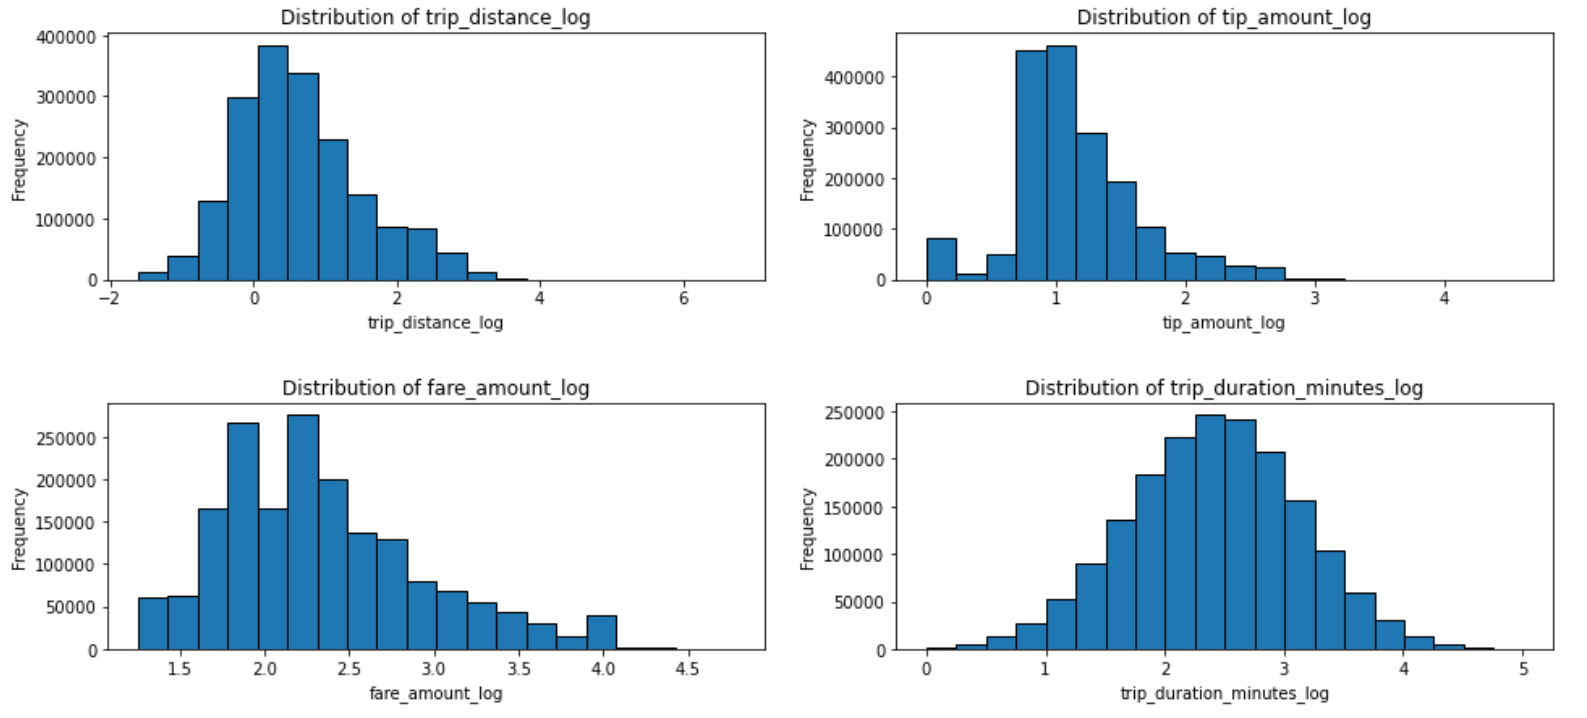
\includegraphics[width=1\textwidth]{plots/loged_distribution.png}
    \centering
    \caption{Distribution of log(numeric feature in taxi data)} % refer to this image as (Figure 1)
\end{figure}


After transformation, from figure 2, we see most trips cover a moderate distance, falling within the range of 0.75 to 1.75 which correspond to 2.117 to 5.7546 miles (by take inverse log). These trips also exhibit a duration spanning from 5 to 26 minutes. This pattern indicates that a significant number of passengers opt for taxi rides for mid-range distances.


\subsection{feature correlations with gasoline}
% Examining the correaltions
From figure 3, notably, gasoline price displays a strong positive correlation with week number (0.89), implying potential temporal trends in fuel costs. However, it seems like weekly average gasoline price has very limited correlation on taxi demand/trip count, hence we will stop investigate this feature. 

Focusing on our target interest of tip amount, we notice that log(tip\_amount) was positively correlated with log of trip distance, period and fare. This could suggest customer willing to offer higher tip for longer trips. 
\begin{figure}[h]
    % change the scale multiplier to make the figures smaller or larger
    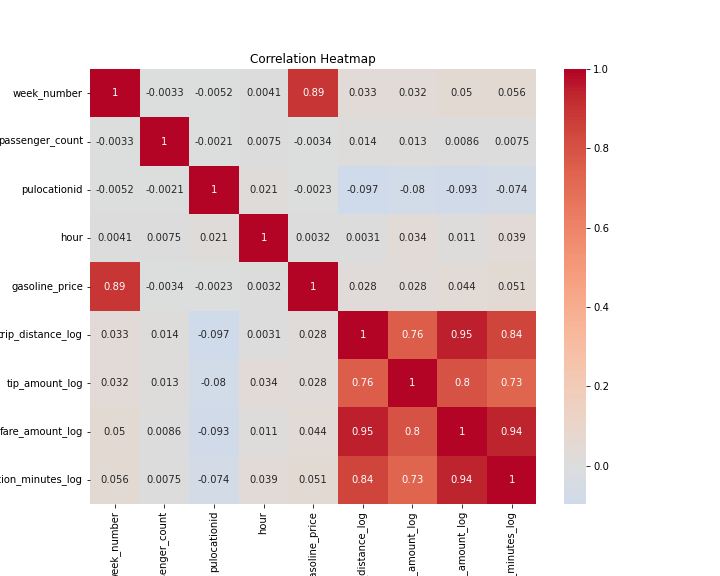
\includegraphics[width=0.80\textwidth]{plots/correlation_heatmap.png}
    \centering
    \caption{Correlation matrix for numeric features} % refer to this image as (Figure 1)
\end{figure}

\subsection{Hourly taxi data}
Observing Figure 4, taxi demand during the late-night period (0am to 6am) is lower compared to other times. Interestingly, the average tip amount and fare amount both peak between 4 am and 5 am. This phenomenon could indicate passenger's willingness to provide higher tips during this timeframe. However, the higher average might also be attributed to the limited data available, as the trip count during these hours is significantly lower compared to other times, potentially skewing the average.
\begin{figure}[h]
    % change the scale multiplier to make the figures smaller or larger
    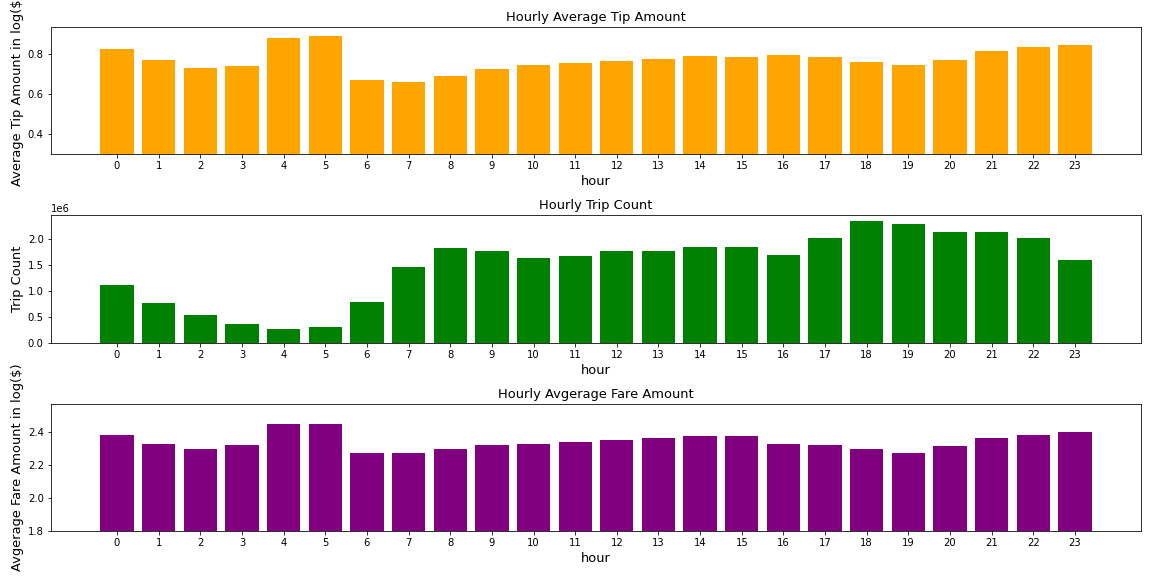
\includegraphics[width=0.95\textwidth]{plots/hourly_analysis.png}
    % this ensures your figures are centered where possible
    \centering
    \caption{Hourly analysis} % refer to this image as (Figure )
\end{figure}

\subsection{Geospatial analysis}
From Figure 5, a clear correlation emerges between taxi demand and pickup locations. From Figure 5 a) we notice pick-up activities are concentrated in Manhattan and key NYC airports—LaGuardia and JFK. Notably, Newark Liberty Airport experiences significant lower demand than the other. This could suggest higher demand at the other airports earlier in the year. However, this observation might be influenced by the possibility of too many record removals during the preprocessing stage.

Moreover, Figure 5 (b)highlights Manhattan as a prime pick-up location, with about 33,378,465 trips originating there, roughly 0.928\% of our total records.

\begin{figure}[h]
    \hspace{-2cm} % Shift the left image towards the left
    \subfigure[Taxi demand/ number of trip record. with airport location labelled ]
    {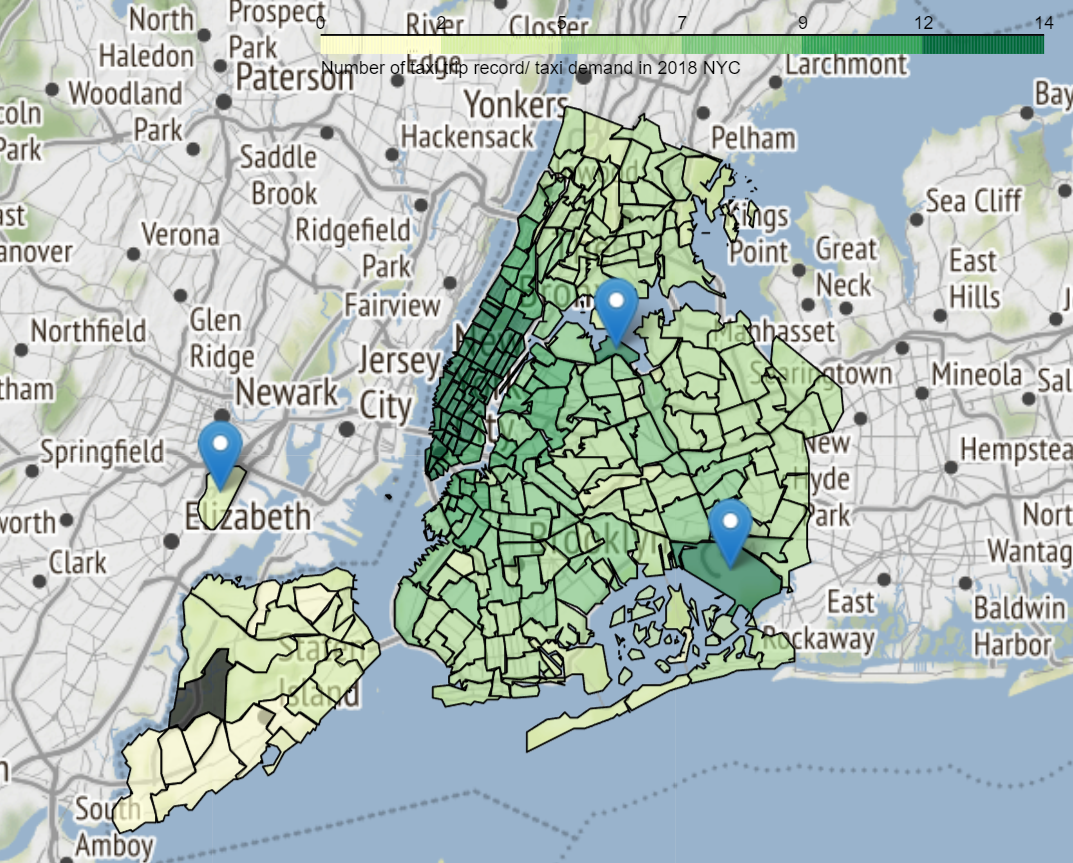
\includegraphics[width=0.5\textwidth]
    {plots/log_taxi_demand.PNG} }  
    \hfill
    \subfigure[Borough Analysis]{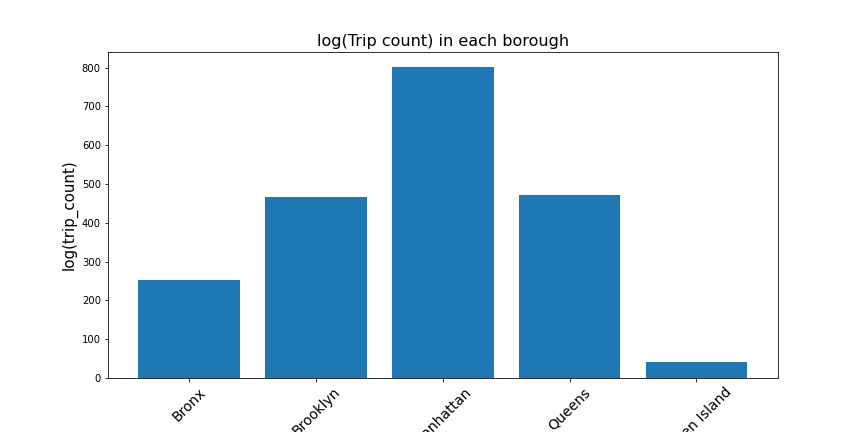
\includegraphics[width=0.68\textwidth]
    {plots/borough_analysis.PNG} }  
    \caption{Geo spatial view of taxi demand and average fare amount in regions.borough} % refer to this image as
\end{figure}


\subsection{Hourly weather analysis}
Examining distributions of weather features, we notice unusual distribution of features like snow and cloud cover in figure 6 a). Like with taxi features, we will apply log transformation to these feature.

In analyzing weather's effect on hourly taxi demand, we've created a correlation coefficient heat map. Surprisingly, only pickup time hour shows a strong positive correlation with hourly taxi demand. Other weather conditions display weak correlations, suggesting minimal linear relationship with taxi demand. However non-linear relationship remain possible.
\begin{figure}[h]
    \subfigure[distribution of weather metric ]
    {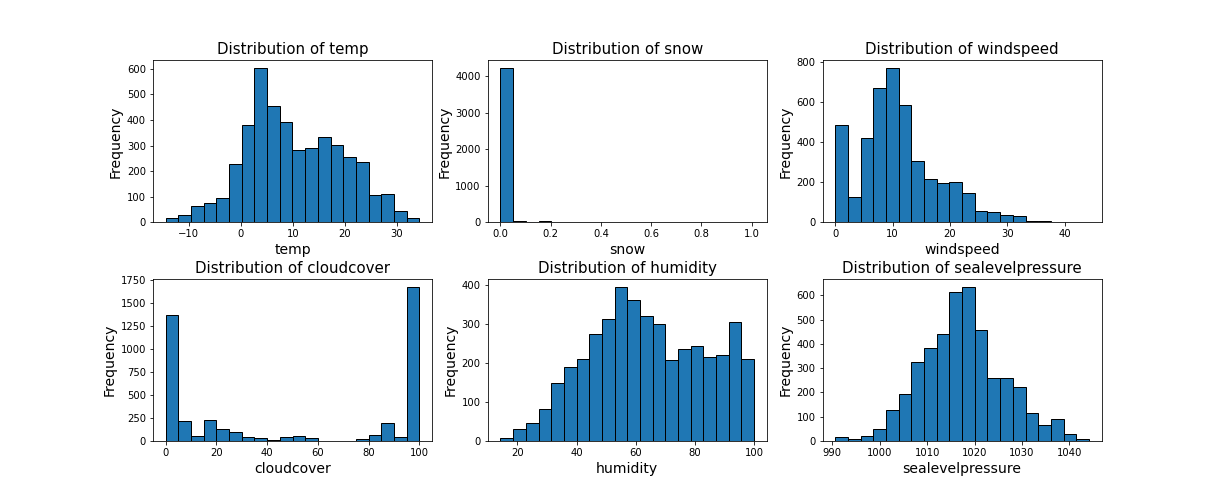
\includegraphics[width=0.9\textwidth]
    {plots/weather_distribution.png} }  
    \hfill
    \subfigure[Correlation between weather conditions and taxi demand hourly]{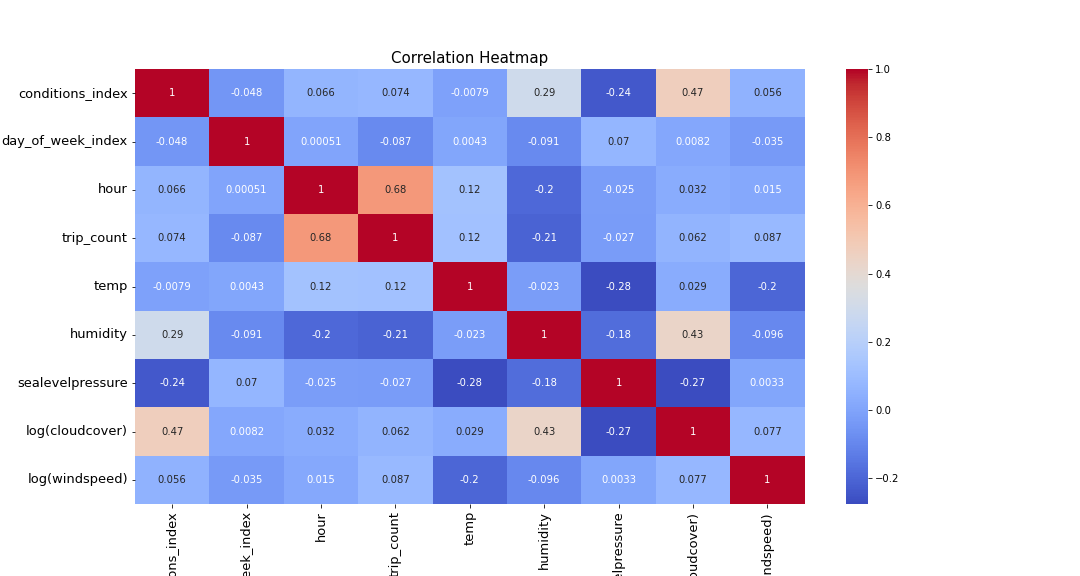
\includegraphics[width=0.8\textwidth]
    {plots/correlation of weathers.png} }  
    \centering
    \caption{Plot with weather data} % refer to this image as
\end{figure}



\section{Modelling}
In this section, we'll use machine learning regression models to predict Manhattan's average hourly taxi demand in March 2019. As Manhattan experiences the highest taxi demand among the boroughs. We'll employ three models: Linear Regression, Random Forest Regression, and K-Nearest Neighbors (KNN)

For feature selection, we'll refer to the correlation coefficient from Figure 6b. Despite the majority having weak linear relationships with our target feature (trip count), we'll use this as a guide to include features with a correlation coefficient close to 0.1. As a result, we'll include conditions\_index, day\_of\_week\_index, hour, temp, log(windspeed), and humidity.


\subsection{Algorithms/Model}
We will employ each model using their default hyperparameters from pyspark and sklearn.
\subsubsection{Linear Regression}
Linear Regression (LR) is suitable for predicting numerical outputs from categorical and numerical predictors \cite{Linear_regression}. Assuming a linear relationship between features and the target (hourly taxi ride demand), independence of demand between different times and homoscedasticity, where residual variance remains constant for any X value.

\subsubsection{Random forest regression}
Random Forest Regression is a supervised learning algorithm that uses ensemble learning method and decision tree regression \cite{random_forest}. It operates under the assumption of observation independence, without requiring explicit linearity between variables or constant residual variance across predictor variable levels. Random Forest Regression is capable of capturing both linear and non-linear relationships between the predictor variables and the target variable. It's well-suited for handling complex relationships and mixed data types.

\subsubsection{KNN}
K-Nearest Neighbors (KNN) is a straightforward and intuitive machine learning algorithm used for classification and regression tasks \cite{KNN}. It predicts based on the closeness of data points in the feature space. KNN Regression assumes that data points with similar features tend to share similar target values in their local vicinity. This technique is suitable for scenarios with continuous target variables and non-linear relationships between features and the target.

\subsection{Result}
Figure 7 (a) presents the predicted results from each model compared to the actual hourly taxi demand data for March 2019. Intriguingly, all models tend to overestimate taxi demand during this period. 

Although it's anticipated that linear regression to have poor performance due to the weak linear relationship between input features and taxi demand, both KNN and Random Forest models also overestimate taxi demand. 

The overestimation of taxi demand is likely attributable to the significant difference in taxi trip records between test data (March 2019) and training data (January to June 2018). With around 3,447,252 records in March 2019 versus an average of 5,563,077.5 taxi records monthly in the training data. This difference in trip records per month can contributes to the model's overestimation.

In addition, external factors like flu outbreaks could potentially happen during the gap period (July 2018 to Feb 2019) which lead to significant fluctuations in taxi demand, resulting in fewer trip records in March 2019.


Addressing average hourly demand under normal conditions, we assume uniform taxi demand monthly. We will sample taxi data record in training data for a consistent count per month (approximately 3-4 million records per month). 

In Figure 7(b), under the assumption of uniform taxi demand monthly, each model performance generally improves, except for linear regression due to its simplistic linear assumption.

Regardless of accuracy from figure 7’s both KNN and Random Forest has manages to capture patterns and trends across the time period which in line with the actual taxi demand pattern. This information can guide Yellow Taxi's service/company and driver scheduling, indicating lower demand from 1am to 6am, a stark increase from 6am to 9am, and a peak demand period from 7pm to 9pm.



\begin{figure}[h]
    \hspace{-3cm} % Shift the left image towards the left
    \subfigure[Prediction vs actual taxi demand]
    {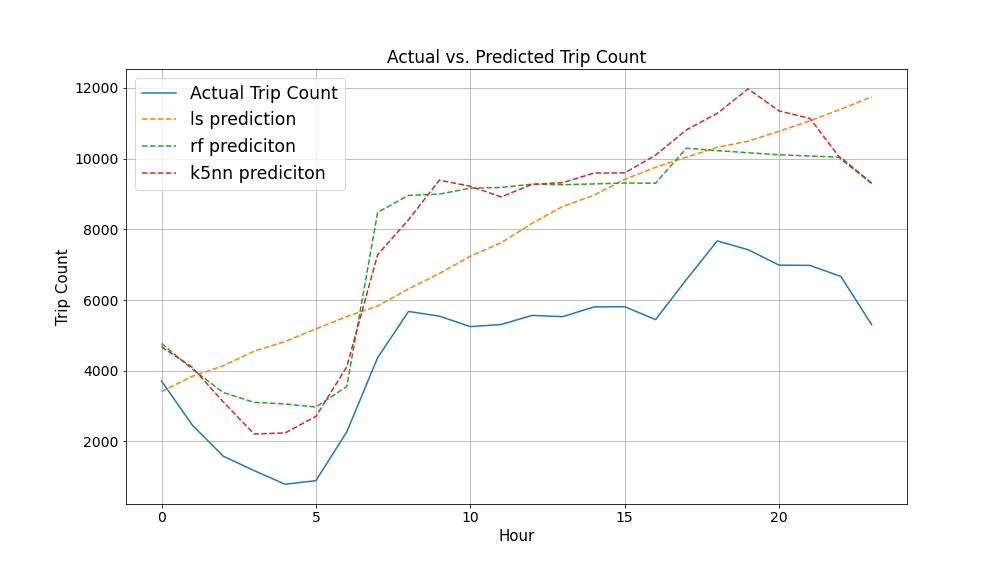
\includegraphics[width=0.7\textwidth]
    {plots/predition.png} }  
    \hfill
    \hspace{-2cm} % Shift the left image towards the left
    \subfigure[prediction vs actual taxi demand with assumption of uniform taxi demand monthly]{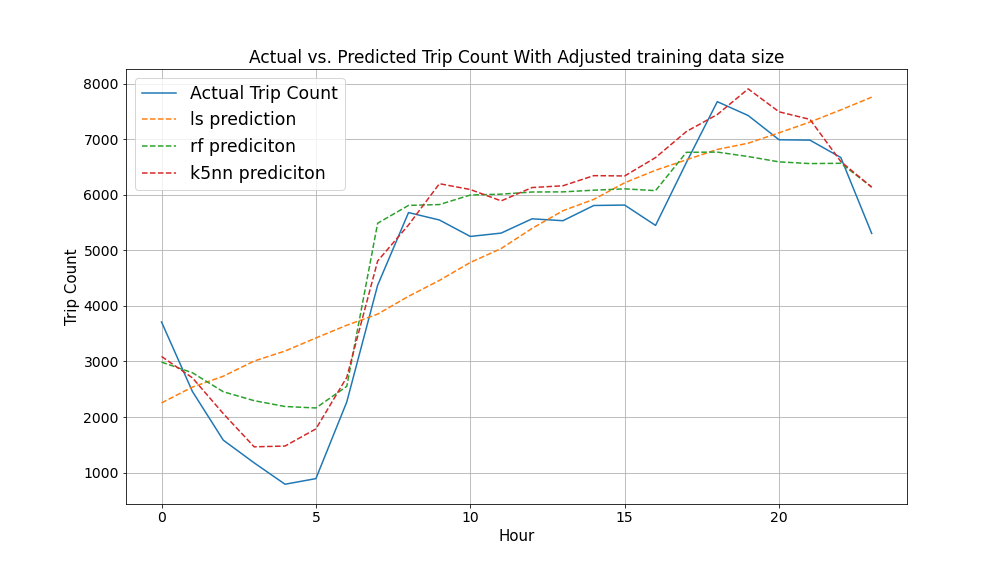
\includegraphics[width=0.7\textwidth]
    {plots/predition_with_adjusted_data_size.png} }  
    \caption{Plot of result of models} % refer to this image as
\end{figure}


\section{Recommendations}
Despite the poor performance model’s prediction, KNN and random forest models were able to capture approximate trends in hourly taxi demand. Given our weather condition feature exhibited limited impact on taxi demand, suggesting the need for more effective predictive variables. Hence, we recommend industry firms to consider developing and enhancing similar models using their own internal data and incorporating additional external factors to obtain a similar model that accurately predicts peak and low periods of taxi demand. This advancement will not only lead to improved service quality but also has the potential to reduce operational costs.

Drawing from the patterns and trends predicted by our models (KNN and random forest) regarding hourly taxi demand, we highly recommend drivers to prioritize their availability during the time frame of 17:00 to 20:00, as this interval consistently demonstrates peak demand. Additionally, we recommend taxi companies to bolster their service offerings  during 6-9am, as our model predicts a significant increase in demand during that time. To ensure a high level of service quality, taxi companies should proactively prepare for this abrupt shift and adjust their operations accordingly.

Our geospatial analysis has revealed a correlation between location ID and taxi demand. Unfortunately, due to the lack of accessible data, we were unable to create a predictive model for location-based taxi demand. We strongly recommend that companies consider building models based on frequent taxi pick-up and drop-off locations, as well as external data such as the number of public transport/numbers of bus stops in that location/area. This can give us an idea of where passengers are likely to request a ride and where additional taxi services are needed.


For drivers seeking to receive higher tip amounts, our hourly analysis in Figure 4 suggests a strategy approach.  Concentrating on providing taxi service during the early morning hours, around 4-5 am, holds the potential for yielding the highest average tip amounts compared to other times. However, it's important to recognize that taxi demand is very limited during this period. While the potential for higher tips exists, there might be fewer available passengers.


If a driver's goal is maximizing earnings, we recommend concentrating on taxi trips between 18-21, the peak demand period. During this time, both taxi demand and the average tip amount are notably high. Balancing tip potential with passenger availability can help drivers optimize their strategy.


\section{Conclusion}
This report examines various aspects of taxi analysis in New York City, including hourly demand, average tips, geographical distribution, and the relationship between weather conditions and gasoline prices with taxi demand. We also perform and evaluate machine learning models linear regression, random forest, and knn models to predict hourly taxi demand in Manhattan during March 2019 based on 2018 data. Despite lower accuracy, these models provided insights into demand trends across different time periods.

For future research, it's worth exploring advanced feature engineering techniques or explore more external data (feature). The lower performance of the linear regression model may be attributed to the absence of linear relationships among numerical features and demand.

Furthermore, we intend to delve deeper into geographical location analysis, aiming to uncover specific details that influence taxi demand in relation to various locations. This investigation will allow us to identify the factors that contribute to the variability in taxi demand based on different geographic areas.

\clearpage

\printbibliography

\end{document}